\documentclass[english,10pt, compress]{beamer}
%\documentclass[english,10pt, compress, handout]{beamer}
\usepackage{mathptmx}
\usepackage[T1]{fontenc}
\usepackage[latin9]{inputenc}
\usepackage{color}
\usepackage{array}
\usepackage{multirow}
\usepackage{amsmath}
\usepackage{amssymb}
\usepackage{fancyvrb}
\makeatletter

%%%%%%%%%%%%%%%%%%%%%%%%%%%%%% LyX specific LaTeX commands.
\newcommand{\noun}[1]{\textsc{#1}}
%% Because html converters don't know tabularnewline
\providecommand{\tabularnewline}{\\}

%%%%%%%%%%%%%%%%%%%%%%%%%%%%%% Textclass specific LaTeX commands.
 % this default might be overridden by plain title style
 \newcommand\makebeamertitle{\frame{\maketitle}}%
 \AtBeginDocument{
   \let\origtableofcontents=\tableofcontents
   \def\tableofcontents{\@ifnextchar[{\origtableofcontents}{\gobbletableofcontents}}
   \def\gobbletableofcontents#1{\origtableofcontents}
 }
 \long\def\lyxframe#1{\@lyxframe#1\@lyxframestop}%
 \def\@lyxframe{\@ifnextchar<{\@@lyxframe}{\@@lyxframe<*>}}%
 \def\@@lyxframe<#1>{\@ifnextchar[{\@@@lyxframe<#1>}{\@@@lyxframe<#1>[]}}
 \def\@@@lyxframe<#1>[{\@ifnextchar<{\@@@@@lyxframe<#1>[}{\@@@@lyxframe<#1>[<*>][}}
 \def\@@@@@lyxframe<#1>[#2]{\@ifnextchar[{\@@@@lyxframe<#1>[#2]}{\@@@@lyxframe<#1>[#2][]}}
 \long\def\@@@@lyxframe<#1>[#2][#3]#4\@lyxframestop#5\lyxframeend{%
   \frame<#1>[#2][#3]{\frametitle{#4}#5}}
 \newenvironment{topcolumns}{\begin{columns}[t]}{\end{columns}}
 \def\lyxframeend{} % In case there is a superfluous frame end


%\setbeamersize{text margin left=.5cm, text margin right=.5cm, text}
% I personally don't think the navigation symbols add anything useful

\hypersetup{colorlinks, urlcolor=blue, linkcolor=magenta}

\usetheme{Warsaw}

\DeclareRobustCommand{\CC}{\hbox{C\hspace{-0.5ex}
                       \protect\raisebox{0.5ex}
                       {\protect\scalebox{0.67}{++}}}}




%\setbeamertemplate{headline}
%{%
%\begin{beamercolorbox}{section in head/foot}
%%\vskip2pt\insertnavigation{\paperwidth}\vskip2pt
%\end{beamercolorbox}%
%}

\newcommand{\Emph}[1]{\textcolor{magenta}{{#1}}}


\usefonttheme{serif}
%\usefonttheme{stillsanserifsmall}
\setbeamercovered{transparent}

\makeatother

\usepackage{babel}
\begin{document}





\title[\CC11]{Modern \CC Basics}


\subtitle{Standard Data Structures and Algorithms}

\author{Dave~Steffen \\
{\tiny with a lot of help
from the \CC Deities.}}

\titlegraphic{
\includegraphics[scale=0.1]{../SciTecLogo.jpeg}}

\institute{SciTec Inc.}


\makebeamertitle






\AtBeginSubsection[]{

  \frame<beamer>{

    \frametitle{Outline}

    \tableofcontents[currentsection,currentsubsection]

  }

}



%\beamerdefaultoverlayspecification{<+->}


\lyxframeend{}\lyxframe{Outline}

\tableofcontents{}




\lyxframeend{}

%%%%%%%%%%%%%%%%%%%%%%%%%%%%%%%%%%%%%%%%%%%%%%%%%%%%%%%%%%%%%%%%%%%%%%
%%%%%%%%%%%%%%%%    SLIDES     %%%%%%%%%%%%%%%%%%%%%%%%%%%%%%%%%%%%%%%
%%%%%%%%%%%%%%%%%%%%%%%%%%%%%%%%%%%%%%%%%%%%%%%%%%%%%%%%%%%%%%%%%%%%%%

\section{Class Extensions}

\section{Intro: \CC11}

\lyxframeend{}\subsection[\CC 11]{{\CC 11} high points}


\begin{frame}[fragile,t]
\frametitle{\CC11 : Major Changes}

\begin{itemize}

  \item \textquotedblleft{}\CC11 feels like a new language.\textquotedblright{} --- Bjarne Stroustrup
    \pause{}

  \item \textasciitilde{}10 features pervasively change \CC\ coding
    syle, idioms, and guidance.
    \pause{}
    {\scriptsize
    \begin{enumerate}
    \item \Emph{nullptr}
    \item \Emph{auto}
    \item \Emph{initializer lists}
    \item \Emph{range-based for loop}
    \item smart pointers
    \item lambdas
    \item move semantics
    \item Class support / extensions
    \item atomic operations / threading
    \item enum class
    \end{enumerate}
}
\end{itemize}

%}
%\end{columns}
\end{frame}

\lyxframeend{}


\begin{frame}[fragile]
\frametitle{\CC11 References}
\framesubtitle{E.G., where Dave stole all this material from}
\begin{itemize}
  \item New books to update style, idioms and guidance:
    \begin{itemize}
    \item \noun{What:} T\CC~PL 4th Ed (Stroustrup) now available

    \item \noun{Why and How}: Style (Meyers) -- ``Effective Modern
      \CC'',  2014.

    \item \noun{Thou Shalt}: \CC\ Coding Standards (Sutter \&
    Alexandrescu, 2005) updated by an extensive website \url{https://isocpp.org/faq}.

    \end{itemize}
\end{itemize}
\end{frame}
%% \lyxframeend{}




%% \begin{frame}[fragile,t]
%% \frametitle{\CC\ Standards through the ages}
%% \begin{description}
%% \item[1985]: First Commerical Release, T\CC~PL, 1st Ed
%% \item[1991]: T\CC~PL, 2nd Ed, added templates and exceptions
%% \item[1997]: T\CC~PL, 3rd Ed, introduced ISO standard, added STL
%% \item[1998]: ISO \CC Standard (``\CC 98'')
%% \item[2003]: \CC 03 (``bug fix'' ISO Standard)\par
%% \item[2007]: TR1 (library additions): shared\_ptr, hash tables
%% \item[2011]: \CC 11, major revisions (what we're talking about today)
%% \item[2013]: Complete \CC11 implementations (GCC 4.8, CLANG 3.2)
%% \item[2014]: \CC 14   ``Bug fix'' to \CC11
%% \item[2017]: \CC17 New stuff; complete implementation in GCC 7
%% \item[2020]: \CC20 (?) In progress
%% \end{description}
%% \end{frame}


%% \lyxframeend{}%\lyxframe{\CC11 : Major Changes}








%% \begin{frame}[fragile]
%% \frametitle{\CC11 References}
%% \framesubtitle{E.G., where Dave stole all this material from}

%% \begin{itemize}
%% \item {\bf The} \CC\ Web Page: {\url{http://isocpp.org}}.  Has links to the actual standard document, blogs, etc.
%%       \begin{itemize}
%%       \item The FAQ at {\footnotesize \url{https://isocpp.org/faq}} has a section devoted to \CC11 features.
%%       \end{itemize}
%% \item GoingNative12 and 13: a bunch of \emph{really} good
%%       talks. {\footnotesize \url{http://herbsutter.com/2012/02/08/going-native-sessions-online/}} and
%%       {\footnotesize \url{http://channel9.msdn.com/Events/GoingNative/2013}}
%% \item CppCon (took over for GoingNative in 2014) talks on YouTube.
%% \item Stroustrup's home page and FAQ. {\footnotesize \url{http://www2.research.att.com/~bs}}
%% \item Herb Sutter's Blog and GOTW {\footnotesize \url{http://herbsutter.com/}}
%% \item C++ Next, particularly Dave Abrahams' discusson of move
%% semantics: {\footnotesize \url{http://web.archive.org/web/20140113221447/http://cpp-next.com/archive/2009/08/want-speed-pass-by-value/}}


%% \item GCC \CC11/14/17 support: {\footnotesize \url{https://gcc.gnu.org/projects/cxx-status.html}}


%% \end{itemize}


%% \end{frame}



%% \begin{frame}[fragile]
%% \frametitle{The rest of this talk}
%% \framesubtitle{``Hitting the high points''}

%% \begin{itemize}

%%         \item auto
%%         \item uniform initialization / initializer lists
%%         \item range-based for loops
%%         \item nullptr
%% %        \item Class extensions
%% %        \item lambdas (and sermon on standard containers and algorithms)
%% %        \item move semantics
%% %        \item smart pointers (and sermon on RAII, SESE, etc)
%% \end{itemize}

%% \end{frame}

\section{Standard C++ Containers}
%%%%%%%%%%%%%%%%%%%%%%%%%%%%%%%%%%%%%%%%%%%%%%%%%%%%%%%%%%%%%%%%%%%%%%
%%%%%%%%%%%%%%%%%%%%%%%%%%%%%%%%%%%%%%%%%%%%%%%%%%%%%%%%%%%%%%%%%%%%%%
%%%%%%%%%%%%%%%%%%%%%%%%%%%%%%%%%%%%%%%%%%%%%%%%%%%%%%%%%%%%%%%%%%%%%%

\begin{frame}[fragile]
\frametitle{Data Structures in the Standard Library}
\framesubtitle{}
\begin{columns}[t]
\column{.5\textwidth}
Stepanov's STL provided 7 standard data structures,
\begin{itemize}
\item vector
\item list
\item deque
\item set and multiset
\item map and multimap
\end{itemize}
with three container adapters:
\begin{itemize}
\item stack
\item queue
\item priority\_queue
\end{itemize}

\column{.5\textwidth}

C++11 adds several more:
\begin{itemize}
\item array
\item forward\_list
\item unordered\_set and unordered\_multiset
\item unordered\_map and unordered\_multimap
\end{itemize}
\end{columns}

\end{frame}
%%%%%%%%%%%%%%%%%%%%%%%%%%%%%%%%%%%%%%%%%%%%%%%%%%%%%%%%%%%%%%%%%%%%%%
%%%%%%%%%%%%%%%%%%%%%%%%%%%%%%%%%%%%%%%%%%%%%%%%%%%%%%%%%%%%%%%%%%%%%%
%%%%%%%%%%%%%%%%%%%%%%%%%%%%%%%%%%%%%%%%%%%%%%%%%%%%%%%%%%%%%%%%%%%%%%
\begin{frame}[fragile]
\frametitle{Data Structures in the Standard Library}
\begin{itemize}
\item Defined types: value\_type, reference, size\_type, etc
\item Iterators:  iterator, const\_iterator, possibly others
\item \texttt{begin, end, cbegin, cend} methods return iterators that
  span the contents.
\item \texttt{size\_t size() const} returns the number of elements
\item \texttt{swap(a,b)} is defined
\end{itemize}

Containers also contain custom or specific methods as appropriate.

\begin{quotation}
``As experienced and sophisticated software engineers, of course, we're
supposed to pooh-pooh ``implementation details,'' but if Einstein is
right and God is in the details, reality requires that we sometimes
get religion'' -- Scott Meyers (on std::string implementations)
\end{quotation}

\end{frame}

%%%%%%%%%%%%%%%%%%%%%%%%%%%%%%%%%%%%%%%%%%%%%%%%%%%%%%%%%%%%%%%%%%%%%%
%%%%%%%%%%%%%%%%%%%%%%%%%%%%%%%%%%%%%%%%%%%%%%%%%%%%%%%%%%%%%%%%%%%%%%
%%%%%%%%%%%%%%%%%%%%%%%%%%%%%%%%%%%%%%%%%%%%%%%%%%%%%%%%%%%%%%%%%%%%%%

\begin{frame}[fragile]
\frametitle{Iterators and Ranges}
\begin{columns}[t]
\column{.7\textwidth}

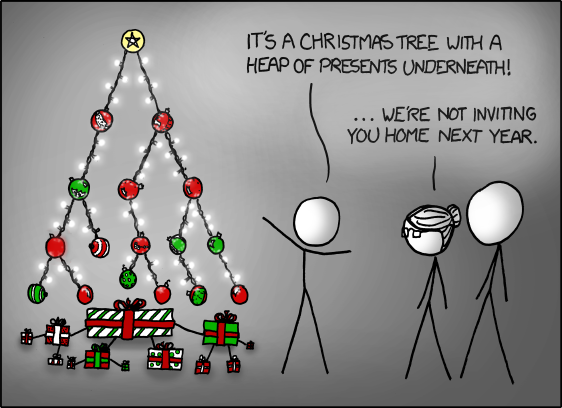
\includegraphics[scale=0.4]{tree.png}

\column{.3\textwidth}<2->
\vskip 24pt
Not only is that terrible in general, but you just KNOW Billy's going to open the root present first, and then everyone will have to wait while the heap is rebuilt.
\end{columns}

\end{frame}



\end{document}
